\documentclass{dhbenelux}

\usepackage{booktabs} % for toprule, midrule, bottomrule in tables
\usepackage{authblk} % for multiple authors and affiliations
\usepackage{graphicx} % to inlcude graphics with \includegraphics

\author[1]{First Author}
\author[2]{Second Author}
\author[2]{Third Author}

\affil[1]{First author's affiliation}
\affil[2]{Second and third authors' affiliation}

\title{Title of the Article}

\begin{document}

\maketitle
\copyrightstatement

\begin{abstract}
    \noindent {[Add an abstract here]}
\end{abstract}

\begin{keywords}
    {[Add keywords here]}
\end{keywords}
\section{Introduction}

This template is intended for articles published in the Digital Humanities in the Benelux Journal.\footnote{See \url{http://journal.dhbenelux.org}} Use this to submit the final version of your manuscript to the journal. The template will ensure your article adheres to the style guidelines of the journal. 

\section{Instructions for preparing your manuscript}

If you are unfamiliar with \LaTeX, there are many online resources with documentation and tutorials on how to use \LaTeX.\footnote{See \url{https://www.overleaf.com/learn/latex/Tutorials}, especially the Learn \LaTeX\ in 30 mintes: \url{https://www.overleaf.com/learn/latex/Learn_LaTeX_in_30_minutes}} 
%
There are specific instructions for preparing your article for the DH Benelux Journal.\footnote{See \url{http://journal.dhbenelux.org/submission/preparing-the-final-version-of-your-manuscript/}}.


\section{Working with bibtex references}

The DH Benelux Journal uses bibtex for references and citations. You can cite other work using bibtex keys \citet{maxwell2013qualitative}. Your article should end with a section called `References' that includes a link to your bibtex file that contains the bibliographic information of the work you cite (see below). Upon generating the print version with a \LaTeX\ engine, references to the cited works are included. 

\section{Adding figures and tables}

This section has two sub-sections.

\subsection{Adding figures}

\begin{figure}
% Use center to align a figure or table to the middle of the text column
\begin{center}
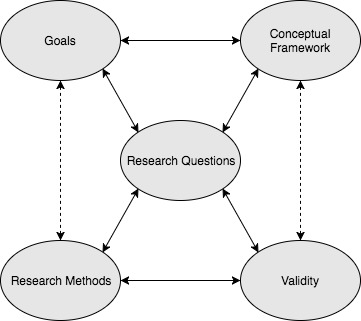
\includegraphics[width=0.6\linewidth]{Images/Maxwell-conceptual-model.jpg}
\end{center}
\caption{This is where the caption of the figure goes. Remember, figure captions go below the figure.}
\label{fig:model_maxwell}
\end{figure}

If you include figures or tables, use reference keys (e.g. Figure~\ref{fig:model_maxwell}), to create an unambiguous reference from the text to each figure and table, e.g. to Table~\ref{tab:groups}.


\subsection{Adding tables}

\begin{table}[tbp!]
\centering
\caption{Table caption. Captions for tables go above the table, unlike for figures.}
\label{tab:groups}
\begin{tabular}{| l | l | l |}
\toprule
 This   & is the  & header row \\
\midrule
 1 & 2 & this is a cell in the first row \\
 3 & 4 & this is a cell in the second row \\
\bottomrule
\end{tabular}
\end{table}



% The reference list will be generated automatically based on the keys 
% you use in your article and their metadata in the bibtex file
\bibliography{references}

\end{document}
